\documentclass[11pt,a4paper]{report}
\usepackage{graphicx} 
\usepackage{setspace}
%\usepackage{microtype}
\usepackage{textcase}
\usepackage{tocloft}
\usepackage{caption}
\usepackage{float}
\usepackage{makecell}
\usepackage[a4paper,top=2.5cm,bottom=2.5cm,left=3cm,right=2.5cm]{geometry}
\usepackage{enumitem}
\usepackage{adjustbox} 
\usepackage{amsmath}
\usepackage[catalan]{babel}
\usepackage{csquotes}
\usepackage[style=numeric, backend=bibtex, sorting=none]{biblatex}
\addbibresource{references.bib}
\usepackage{hyperref}

\onehalfspacing
\setlength{\parindent}{0pt}
\setlength{\parskip}{6pt}

\newcommand{\titolTFG}{Sistema digital de gestió per a protectores i refugis d'animals
}

\usepackage{colortbl}
\newcommand{\yescell}{\cellcolor{lightblue}Sí}

\newcommand{\portada}{
\begin{titlepage}
    \centering
    \vspace*{0.5cm}
    
\includegraphics[height=2.5cm]{logo-fiblletres.png}
    \hspace*{0.5cm}
    
\includegraphics[height=2.5cm]{Logo_UPC.svg.png}

    \vspace{0.8cm}
    {\large\textsc{Universitat Politècnica de Catalunya}\par}
    \vspace{0.1cm}
    {\normalsize Facultat d'Informàtica de Barcelona\par}
    
    \vspace{0.8cm}
    {\small\textsc{Treball de Fi de Grau en Enginyeria Informàtica}\par}
    \vspace{0.1cm}
    {\normalsize Especialitat en Enginyeria del Software\par}
    
    \vfill
    {\LARGE\bfseries \titolTFG \par}
    \vspace{0.5cm}
    {\Large\textit{Dídac Dalmases Valcárcel}\par}
    \vspace{0.5cm}
    {\normalsize Directora: MARÍA JOSÉ CASAÑ GUERRERO\par}
    \vspace{0.5cm}
    {\normalsize Tutora: CAROLINA CONSOLACIÓN SEGURA\par}
    \vfill
    18/03/2026
\end{titlepage}
}

\usepackage{xcolor}
\definecolor{tocblue}{RGB}{0, 70, 180}
\definecolor{oceanblue}{RGB}{15, 64, 143}
\definecolor{lightblue}{RGB}{189, 228, 255}

%chapter entries bold and blue
\setlength{\cftaftertoctitleskip}{6pt}
\setlength{\cftafterloftitleskip}{6pt}
\setlength{\cftafterlottitleskip}{6pt}

\setlength{\cftbeforetoctitleskip}{0pt}
\setlength{\cftbeforeloftitleskip}{0pt}
\setlength{\cftbeforelottitleskip}{0pt}

\setlength{\cftbeforechapskip}{6pt}

%start section from 1
\renewcommand{\thesection}{\arabic{section}}
\setcounter{secnumdepth}{3}

%macro for user story tables
\newcommand{\HU}[9]{%
\begin{table}[H]\centering\small\renewcommand{\arraystretch}{1.3}%
\begin{tabular}{|l|p{4.5cm}|p{4.5cm}|}\hline
\rowcolor{oceanblue}\textcolor{white}{\textbf{Història d'Usuari}} & \multicolumn{2}{l|}{\textcolor{white}{#2}} \\\hline
\textbf{Objectiu} & \multicolumn{2}{l|}{#1} \\\hline
\rowcolor{gray!10}\textbf{Puntuació} & \textbf{Frontend} & \textbf{Backend} \\\cline{2-3}
& #3 & #4 \\\hline
\textbf{Prioritat} & \multicolumn{2}{l|}{#5} \\\hline
\rowcolor{oceanblue}\multicolumn{3}{|l|}{\textcolor{white}{\textbf{Descripció}}} \\\hline
\multicolumn{3}{|p{12.5cm}|}{\textbf{Com a} #6, \newline \textbf{Vull} #7, \newline \textbf{Per tal de} #8.} \\\hline
\rowcolor{oceanblue}\multicolumn{3}{|l|}{\textcolor{white}{\textbf{Criteris d'Acceptació}}} \\\hline
\multicolumn{3}{|p{12.5cm}|}{\begin{enumerate}[leftmargin=0.5cm,topsep=2pt,parsep=0pt,itemsep=3pt] #9 \end{enumerate}} \\\hline
\end{tabular}\caption[Història d'usuari: #2]{Història d'usuari de: #2. Font: Elaboració pròpia}\label{tab:hu_#1}\end{table}%
}

\begin{document}
\portada

\renewcommand{\contentsname}{Índex}
\renewcommand{\listfigurename}{Índex de figures}
\renewcommand{\listtablename}{Índex de taules}
\renewcommand{\figurename}{Figura}
\renewcommand{\tablename}{Taula}
\renewcommand{\bibname}{Referències}

\captionsetup[figure]{font=it}
\tableofcontents
\newpage
\listoffigures
\newpage
\listoftables
\newpage
\section{Introducció}
El projecte \titolTFG és un Treball de Fi de Grau (TFG) del grau d'Enginyeria Informàtica, més en concret de l’especialitat d’Enginyeria del Software, de la Facultat d’Informàtica de Barcelona (FIB) de la Universitat Politècnica de Catalunya (UPC). S’ha realitzat amb la modalitat A i és dirigit per la María José Casañ Guerrero.

\subsection{Context} \label{sec:context}
L’abandonament i el maltractament animal són problemàtiques que porten presents a la nostra societat des de l’inici de la domesticació de les primeres espècies. Aquests animals, que prèviament eren amb una família o han estat abandonats en néixer pels seus amos, no tenen un futur clar al moment en què arriben al carrer, és aquí on es destaca la importància de les protectores i dels refugis d’animals.

Catalunya va arribar a un màxim històric d'abandonaments de gossos i gats durant l'any 2024, superant fins i tot les xifres registrades durant la pandèmia del 2020. Segons l'informe anual "Él Nunca Lo Haría" de la Fundació Affinity \cite{fundacion_affinity_inicio_nodate}, un total de 292.000 gossos i gats (173.000 gossos i 118.000 gats respectivament) van haver de ser recollits per protectores d'animals a tot Espanya, amb Catalunya representant aproximadament el 20\% d'aquests casos.

Cal destacar que aquestes xifres només reflecteixen els animals que efectivament arriben a protectores i refugis oficials. El nombre real d'abandonaments pot arribar a ser superior, ja que no inclou:

\begin{itemize}
    \item Animals que viuen al carrer sense ser detectats
    
    \item Colònies felines sense gestionar

    \item Animals que són recollits per particulars sense registre oficial
    
    \item Casos en zones rurals on no hi ha cobertura de protectores
\end{itemize}

Els animals abandonats que són principalment gats i gossos acaben a protectores i refugis. Aquests són organismes que busquen donar una llar i cuidar-los de manera temporal fins a poder donar-los en adopció. Existeixen centres municipals (CAAC) que reben recursos públics per a dur a terme les tasques i processos que comporta acollir a un animal, i els centres voluntaris i privats. Aquest segon grup, que té més rellevància al projecte, funciona gràcies als voluntaris, les cases d’acollida que tinguin disponibles i els donants. Segons la Fundació per a l'Assessorament i Acció en Defensa dels Animals (FAADA), hi ha un total de 613 centres d’acollida i protectores d’animals \cite{faada_protectoras_nodate} a tota Espanya.

El dia a dia de les protectores no només tracta de l’alimentació i el cuidat bàsic dels animals, sinó que també han de realitzar les gestions mèdiques de cadascun dels animals, portant a terme un seguiment del seu estat des que el recullen fins que el donen en adopció, passant per vacunes, veterinaris i altres processos. També és present tota una part logística que consisteix a obtenir i preparar els materials necessaris per a les instal·lacions que s’utilitzin, les neteges periòdiques, els torns dels voluntaris que hi participin, entre d’altres.  Una altra responsabilitat d’aquestes protectores és l’àmbit legal, com podrien ser els xips i els contractes d’adopció dels animals en acollida. 

Es veu, doncs, una situació que exigeix un nivell d'organització i gestió dels recursos que pot sobrepassar les capacitats dels mètodes més tradicionals utilitzats per protectores petites i mitjanes. La digitalització d'aquests processos no només representa una oportunitat de guanyar eficiència operativa, sinó que es configura com una necessitat crítica per a la supervivència d'aquestes entitats. 

\subsection{Identificació del problema}
La majoria de protectores, ja estiguin registrades oficialment o no, són de mida petita i sobreviuen amb els pocs recursos que tenen. Amb aquest context, l’organització que es fa del dia a dia i la gestió de tot el que comporta dirigir o formar part d’una protectora, es converteix en un aspecte clau per a poder seguir endavant com a entitats sense ànim de lucre. 

Per culpa de la falta d’eines i temps, les protectores i refugis es troben gestionant les feines del dia a dia amb mètodes antiquats, com poden ser fulls de càlcul senzills, documents físics sense un clar ordre i missatges de text per poder comunicar-se entre els participants. Així doncs, es crea un gran problema de falta de traçabilitat, on la informació queda dispersa per l’associació a més de patir el risc de perdre’s totalment si no està correctament enregistrada i és dependent del factor humà.

Relacionat amb el punt anterior, la gestió dels voluntaris és un altre pilar de les protectores que necessita està ben organitzat. Si no s’utilitza una aplicació especialitzada, aquest procés es realitza a través d'eines de missatgeria com pot ser WhatsApp, creant una dificultat afegida a l’hora d'enregistrar les tasques de cada voluntari, mesurar la contribució de cadascun i de nou, perdent molta traçabilitat en les accions del dia a dia.

Totes aquestes limitacions tenen un impacte directe en l’objectiu de les protectores: Els processos d’adopció s’allarguen més del que hi hauria per la gestió manual de sol·licituds, es perden adoptants potencials, i la falta d’una visió global de l’estat dels animals i les tasques a realitzar provoquen una presa de decisions ineficient. En definitiva, la falta de digitalització no només genera ineficiències, sinó que compromet la capacitat real de les protectores per salvar vides animals i millorar-les.


\subsection{Actors implicats}

Els stakeholders o parts interessades són aquelles persones o conjunt de persones que estan implicades directament o indirectament amb el projecte. Identificar-los correctament permet definir els requisits amb una precisió més elevada i ajuda a entendre el context del treball.

\begin{itemize}
    \item \textbf{Protectores i refugis d’animals}: Entitats sense ànim de lucre que acullen animals abandonats i que utilitzaran el sistema per gestionar les seves operacions diàries. Són els clients o entitats beneficiàries directes del projecte.
    
    \item \textbf{Gestors i coordinadors de protectores}: Usuaris encarregats de l'administració de l'entitat. Utilitzaran el sistema per validar sol·licituds d'adopció, assignar tasques, gestionar la documentació i organitzar els recursos del refugi.
    
    \item \textbf{Voluntaris de protectores}: Usuaris que fan el treball de camp diari al refugi. Utilitzaran l'aplicació mòbil per consultar les tasques pendents (alimentació, neteja, medicació), llegir les fitxes dels animals i actualitzar-ne l'estat en temps real.
    
    \item \textbf{Adoptants}: Qualsevol individu que vulgui adoptar un animal i interactuï amb el sistema a través d’internet, utilitzant el portal web per cercar animals, enviar sol·licituds i signar contractes.
    
    \item \textbf{Directora del TFG}: La directora dirigirà i supervisarà el projecte durant la seva durada, donant suport quan sigui necessari i vetllant per l'assoliment dels objectius acadèmics.
    
    \item \textbf{Desenvolupador}: L'autor del projecte, encarregat de dissenyar i implementar el sistema digital amb l’objectiu de complir amb els requisits establerts, així com d'elaborar la present memòria escrita.
\end{itemize}

\subsection{Conceptes previs}
\begin{itemize}
    \item CAAC \cite{covb_centres_nodate}
    
    Instal·lacions, generalment de titularitat pública o municipal, dedicades a la recollida d'animals perduts o abandonats, amb l'objectiu de fomentar-ne l'adopció i promoure la tinença responsable.
    
    \item MVP \cite{atlassian_minimum_nodate}
    
    Versió inicial d'un producte amb les característiques justes i suficients per ser llançat al mercat, amb l'objectiu de validar idees.
    
    \item Monorepo \cite{sonarsource_what_nodate}
    
    És una estratègia d'arquitectura on el codi font de múltiples projectes i aplicacions, encara que siguin independents s'emmagatzema dins d'un únic repositori de control de versions.
    
    \item JWT \cite{auth0_json_nodate}

    Estàndard per transmetre informació d'autenticació de forma segura entre client i servidor mitjançant tokens signats digitalment, eliminant la necessitat de mantenir sessions al servidor.
    \item RBAC \cite{entrust_what_nodate}
    
    És un mecanisme de seguretat que restringeix l'accés als recursos d'un sistema basant-se en els rols que tenen els usuaris dins de l'organització (per exemple: Administrador, Voluntari, Gestor).
\end{itemize}

\newpage
\section{Justificació}
Per poder entendre els motius d’aquest projecte, cal avaluar si aquest aporta innovació respecte a les solucions ja existents. Amb aquest objectiu, es realitzarà un estudi del mercat avaluant les característiques presents, les mancances i les limitacions respecte al problema comentat anteriorment. Finalment, es compararà amb la solució proposada, avaluant la viabilitat d’aquesta i el valor que aporta respecte a les altres.

\subsection{Anàlisi del mercat}
Les aplicacions per organitzar protectores i refugis d’animals existeixen des de fa molt temps, a causa de ser un problema recurrent i extern a l’avanç de les tecnologies. Així i tot, no hi ha un gran nombre, ja que és un domini que no té la capacitat de monetització ni el potencial econòmic com d’altres. Aquest estudi es centra en solucions orientades a protectores d'animals sense ànim de lucre, caracteritzades per treballar amb voluntaris, cases d'acollida temporal i finançament via donacions.

Abans d'avaluar les solucions existents, cal definir el perfil de la solució que es busca: 
una eina gratuïta, de codi obert, accessible a usuaris sense formació tècnica, que integri 
en una única plataforma la gestió dels animals, els voluntaris i el procés d'adopció complet, 
i que estigui orientada a protectores petites i mitjanes europees. Aquest perfil servirà de 
referència per avaluar les mancances de cada alternativa analitzada.

\subsubsection[ShelterLuv]{ShelterLuv \cite{shelterluv_shelterluv_nodate}}
ShelterLuv és un software orientat a cobrir i automatitzar totes les necessitats d'una protectora d'animals. Es tracta d'una empresa consolidada amb diversos clients, que proclama haver aconseguit 53 milions de dòlars per als seus usuaris a través de donacions. Entre les seves funcionalitats destaquen l'inici i el seguiment del procés d'adopció, la creació i organització de tasques per a cada animal, un resum mèdic detallat i l'accés a una base de dades pròpia per als microxips. Malgrat l'amplitud de les seves funcionalitats, el fort acoblament amb el marc legal i administratiu dels Estats Units i l'enfocament en grans organismes amb una organització de base ja consolidada en limiten considerablement l'aplicabilitat per a protectores petites i mitjanes europees.

\subsubsection[Miwuki Pet Shelter / Miwuki Pet Center]{Miwuki Pet Shelter / Miwuki Pet Center \cite{miwuki_miwuki_nodate}}
Miwuki és la solució amb més rellevància en l'àmbit nacional espanyol. Es basa en dos mòduls: un per presentar els animals en adopció i les protectores que els gestionen, i un altre per a l'administració interna. Entre les seves característiques destaquen la gestió de l'historial de cada animal, la publicació automàtica en múltiples portals d'adopció i la gestió de les fitxes dels adoptants. No obstant això, deixa de banda activitats quotidianes clau com l'organització dels voluntaris i el manteniment de les instal·lacions. A més, l'aplicació mòbil per a les protectores queda limitada a la visualització de dades, desaprofitant el potencial que hauria de tenir com a eina de camp.

\subsubsection[Shelter Manager]{Shelter Manager \cite{sheltermanagercom_shelter_nodate}}
Shelter Manager és un software web adaptat a mòbil i ordinador que inclou la gestió d'animals i persones, el control d'entrades i sortides, la generació automàtica d'informes i l'apartat econòmic. Ofereix un alt grau de personalització, permetent afegir camps i categories a la protectora. Tanmateix, aquest nivell d'exhaustivitat té un cost: la interfície d'usuari és sobrecarregada i poc intuïtiva, cosa que genera una corba d'aprenentatge elevada. Per a protectores petites o mitjanes amb personal voluntari i poca experiència tècnica, aquesta complexitat es converteix en una barrera d'entrada real, no en un avantatge.

\subsubsection[AnimalsFirst]{AnimalsFirst \cite{animalsfirst_track_nodate}}
AnimalsFirst és una solució de gestió en el núvol que actua com a SaaS amb una interfície polida i accessible. Té com a objectiu reduir la càrrega administrativa d'un refugi centralitzant-ho tot en una única aplicació. Com a punts forts destaquen un seguiment mèdic amb alertes automàtiques per a vacunes i tractaments pendents, i una integració senzilla cap a altres plataformes d'adopció i xarxes socials. Tot i ser una de les opcions més modernes, no cobreix la gestió operativa interna de la protectora, com l'organització dels voluntaris o les tasques de manteniment, aspectes fonamentals per al dia a dia d'una entitat d'aquest tipus.

\subsubsection[24PetShelter Chameleon]{24PetShelter Chameleon \cite{24pet_bringing_nodate}}
Chameleon és una de les solucions que ofereix 24Pet per a les protectores d'animals, centrada específicament en la gestió i telemetria dels voluntaris i encarregats. Permet també gestionar l'inventari i crear campanyes de donacions, incorporant un alt grau de personalització per a organitzacions complexes. El problema principal no rau en les funcionalitats individuals, sinó en el model: obtenir una gestió completa de la protectora obliga a contractar múltiples mòduls no centralitzats, amb un cost acumulat significativament superior al de les alternatives. Per a entitats amb recursos limitats, aquesta fragmentació és un obstacle difícil de justificar.

\subsection{Conclusions}
L'anàlisi realitzada mostra un patró comú entre les solucions estudiades: cadascuna resol bé una part del problema, però cap no l'aborda en la seva totalitat. Les plataformes més completes, com ShelterLuv o Shelter Manager, arrosseguen limitacions d'accessibilitat, ja sigui per barreres culturals i econòmiques o per una interfície que penalitza l'usuari no tècnic. Les més modernes i accessibles, com AnimalsFirst o Miwuki, sacrifiquen la gestió operativa interna en favor d'una experiència més polida. I les que intenten cobrir-ho tot, com 24PetShelter, ho fan a través d'un model fragmentat que multiplica el cost i la complexitat.

El resultat és que cap d'elles és una opció viable per a una protectora petita o mitjana europea que necessiti, alhora, gestionar els seus animals, organitzar els voluntaris i oferir un portal d'adopcions modern, tot de forma centralitzada, gratuïta i sense requerir coneixements tècnics. Aquesta és precisament la bretxa que aquest projecte vol cobrir, tal com es recull a la taula comparativa següent.

\begin{table}[H]
    \centering
    \small
    \renewcommand{\arraystretch}{2}
    \begin{tabular}{|l|c|c|c|c|c|c|}
        \hline
        \textbf{Característica} & \cellcolor{oceanblue}\textcolor{white}{\textbf{ShelterLuv}} & \cellcolor{oceanblue}\textcolor{white}{\textbf{Miwuki}} & \cellcolor{oceanblue}\textcolor{white}{\makecell{\textbf{Shelter}\\\textbf{Manager}}} & \cellcolor{oceanblue}\textcolor{white}{\textbf{AnimalsFirst}} & \cellcolor{oceanblue}\textcolor{white}{\textbf{Chameleon}} & \cellcolor{oceanblue}\textcolor{white}{\textbf{TFG}} \\
        \hline
        Portal d'adopcions & \yescell & \yescell & No & \yescell & No & \yescell \\
        \hline
        Interfície moderna & \yescell & \yescell & No & \yescell & No & \yescell \\
        \hline
        Codi obert & No & No & No & No & No & \yescell \\
        \hline
        \makecell[l]{Gestió de\\ tasques diàries} & \yescell & No & \yescell & No & \yescell & \yescell \\
        \hline
        \makecell[l]{Ecosistema\\ col·laboratiu} & No & No & No & No & No & \yescell \\
        \hline
        Gestió d'animals & \yescell & \yescell & \yescell & \yescell & \yescell & \yescell \\
        \hline
    \end{tabular}
    \caption[Resultat de l'anàlisi de mercat]{Resultat de l'anàlisi de mercat. Font: Elaboració pròpia}
    \label{tab:mercat}
\end{table}

Es pot concloure doncs que les solucions existents o bé són de pagament i pensades per a grans organitzacions, o bé cobreixen únicament aspectes parcials de la gestió d'una protectora. Cap d'elles integra en una mateixa plataforma la gestió interna dels animals, incloent-hi l'historial mèdic i els tractaments, l'organització autònoma dels equips de voluntaris mitjançant torns i tasques, i un portal públic d'adopcions que automatitzi tot el procés fins a la signatura del contracte. Veient aquesta oportunitat, aquest projecte neix com una alternativa de codi obert, accessible i adaptada a la realitat de les protectores petites i mitjanes, amb l'objectiu de centralitzar totes aquestes necessitats en una única eina pensada específicament per a aquest domini.

\newpage
\section{Abast}
En aquest apartat definirem els objectius, subobjectius, requisits no funcionals i els possibles obstacles i riscos del projecte.

\subsection{Objectius}
L'objectiu principal d'aquest treball de fi de grau és la creació d'un sistema digital que permeti a les protectores gestionar la feina del seu dia a dia més fàcilment i còmodament, centralitzant les necessitats de cada entitat en una aplicació, a més d'agilitzar els processos d'adopció dels animals a través d'un portal públic d'adopcions. Per assolir aquest objectiu s'han d'assolir els següents subobjectius:

\begin{itemize}
    \item Registrar gossos i gats de múltiples protectores al sistema de forma independent, incloent-hi informació mèdica, tractaments i l'historial de cada animal, centralitzant tota la informació en un únic lloc.
    \item Digitalitzar la gestió dels voluntaris mitjançant torns i tasques assignades, permetent que cada protectora organitzi el seu equip de forma autònoma i faci un seguiment de la participació de cada voluntari.
    \item Gestionar el procés d'adopció complet a través d'un portal públic, des del formulari inicial fins a la signatura del contracte, realitzant un seguiment de cada pas del procés per a totes les protectores registrades al sistema.
    \item Facilitar la col·laboració entre protectores registrades al sistema mitjançant un ecosistema d'intercanvi d'inventari, reduint costos i aprofitant els recursos disponibles entre entitats.
    \item Proporcionar un sistema d'alertes configurable basat en els tractaments dels animals i l'estat de les tasques assignades, adaptat a les necessitats específiques de cada protectora.
\end{itemize}

\subsection{Requisits no funcionals}
\begin{itemize}
    \item NFR1. \textbf{Usabilitat}: La interfície del portal web i de l’aplicació ha de ser fàcil d’utilitzar per a usuaris sense formació tècnica prèvia, habilitant el seu ús per a qualsevol persona.
    \item NFR2. \textbf{Escalabilitat}: El sistema ha de ser capaç de gestionar un increment d’usuaris sense afectar les funcionalitats principals, suportant el creixement progressiu de protectores i usuaris registrats al sistema.
    \item NFR3. \textbf{Privacitat}: El sistema ha de complir de manera estricta amb el Reglament General de Protecció de Dades (RGPD), garantint la confidencialitat i el tractament segur de les dades personals de tots els actors implicats.
    \item NFR4. \textbf{Disponibilitat}: El portal web d’adopcions i les funcionalitats de l’aplicació han d’estar disponibles un 99\% del temps com a mínim.
    \item NFR5. \textbf{Internacionalització}: El sistema ha de tenir l’opció d’escollir idioma entre català i castellà.
    \item NFR6. \textbf{Seguretat}: El sistema ha d'implementar autenticació segura mitjançant tokens (JWT), control d'accés basat en rols (RBAC) i comunicació xifrada (HTTPS) per garantir que cada actor només pugui accedir a les funcionalitats que li corresponen.
\end{itemize}

\subsection{Obstacles i riscos}
Durant el procés del projecte és inevitable l’aparició de problemes que poden perjudicar el desenvolupament del sistema. És important identificar aquests possibles obstacles i riscos per plantejar alternatives en cas de donar-se. A més de la descripció, se'ls  atribueix un grau d’impacte.
\begin{itemize}
    \item \textbf{Data límit d’entrega}: Aquest treball de fi de grau, com tots, està limitat a ser entregat un dia en concret. Aquest és un obstacle que pot provocar que algunes funcionalitats planificades inicialment puguin ser simplificades o descartades. Per minimitzar aquest risc, es prioritzarà crear un MVP amb les funcionalitats nucli del sistema. Impacte: Mitjà.
    \item \textbf{Manca d’accés a usuaris reals per validació}: No realitzar aquest projecte directament amb una protectora durant el desenvolupament podria generar una desalineació amb el sistema resultant i les necessitats reals de les protectores. Per minimitzar aquest risc, s’ha realitzat un estudi previ del funcionament de les protectores i solucions similars ja existents. Impacte: Alt.
    \item \textbf{Falta d’experiència prèvia amb les tecnologies}: L’autor del projecte té una experiència limitada amb les tecnologies que s’utilitzaran per al sistema i amb una arquitectura multiplataforma com pot ser el portal i l’aplicació mòbil. Per mitigar aquest risc, es destinarà una fase inicial a la formació pràctica mitjançant la documentació oficial i el desenvolupament de petites proves de concepte. Impacte: Alt.
    \item \textbf{Bugs}: L’aparició de problemes dins del mateix desenvolupament és inevitable. Aquests bugs i errors poden portar endarreriments a la planificació. Per mitigar-los es realitzaran una sèrie de tests per validar totes les funcionalitats. Impacte: Alt.
\end{itemize}

\newpage
\section{Metodologia de treball}
Aquest apartat descriu la metodologia que s’utilitza per al projecte, detallant-la per parts.

\subsection{Gestió del projecte}
El projecte es realitzarà seguint una metodologia àgil basada en Scrum, adaptada per a un únic desenvolupador. Això implica mantenir l'estructura de sprints com a unitat de planificació i seguiment, però prescindint d’algunes cerimònies pròpies d'un equip. L'eina utilitzada per a la gestió serà Taiga \cite{taiga_your_nodate}, una plataforma de gestió de projectes àgils que permet organitzar el treball en èpiques, històries d'usuari i tasques.

Aquesta metodologia s'adapta bé al projecte, ja que permet dividir la complexitat del sistema en parts manejables sobre les quals iterar progressivament. Així, tot i comptar amb un únic desenvolupador, és possible construir un producte robust de manera ordenada i sostenible.

La planificació s'organitza en tres nivells de granularitat:
\begin{itemize}
    \item \textbf{Èpiques}: Representen els mòduls essencials del sistema de manera general. Cada èpica agrupa un conjunt de funcionalitats relacionades que, en conjunt, conformen una part significativa del producte final.
        \begin{figure}[H]
            \centering
            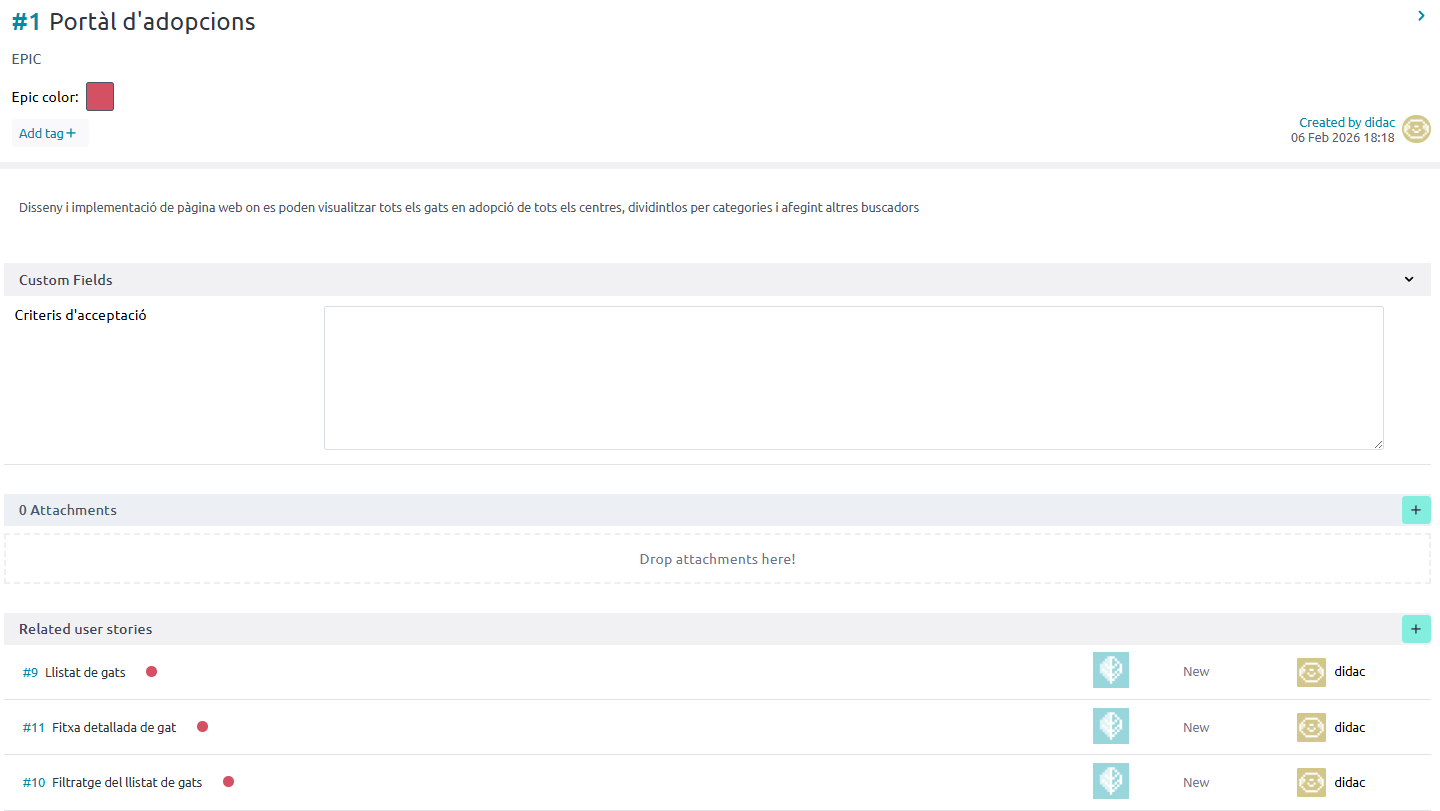
\includegraphics[width=0.8\textwidth]{taiga_epic_example.png}
            \caption[Exemple d'èpica]{Exemple d'èpica. Font: Elaboració pròpia}
            \label{fig:taiga_epics}
        \end{figure}

    \item \textbf{Històries d'usuari}: Dins de cada èpica es troben les històries d'usuari, que descriuen una funcionalitat concreta des del punt de vista de l'usuari final, seguint el format \textit{"Com a [rol], vull [acció] per tal de [benefici]"}. A més, tenen uns criteris d’acceptació a complir per poder considerar-se finalitzades. 
        \begin{figure}[H]
            \centering
            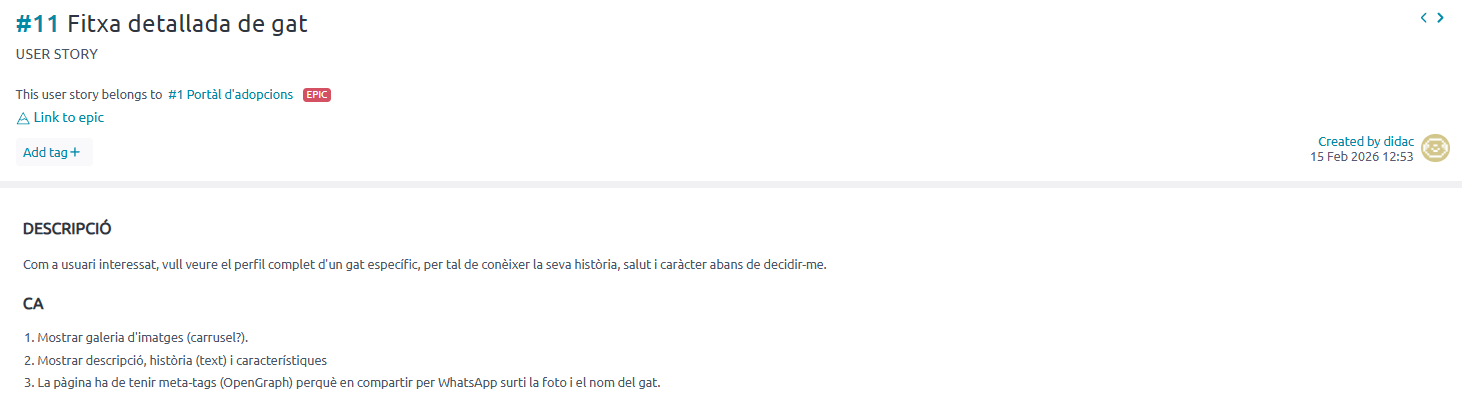
\includegraphics[width=0.8\textwidth]{taiga_userStory_example.png}
            \caption[Exemple d'història d'usuari]{Exemple d'història d'usuari. Font: Elaboració pròpia}
            \label{fig:taiga_userstory}
        \end{figure}
    \item \textbf{Tasques}: Cada història d'usuari es descompon en tasques tècniques concretes que representen el treball real de desenvolupament.
Per validar que els objectius s'assoleixen en cada sprint, s'utilitzen diversos mecanismes de seguiment. 

Cada història d'usuari disposa de criteris d'acceptació que defineixen explícitament quan es considera finalitzada, actuant com a definició de "done". La retrospectiva realitzada al final de cada sprint o release permet avaluar si els objectius planificats s'han assolit i identificar millores per a les iteracions següents.
\end{itemize}

\subsection{Gestió del repositori}
Per dur a terme el control de versions d’aquest projecte s’ha escollit Git \cite{git_git_nodate} mitjançant els servidors i les funcionalitats de GitHub \cite{github_change_nodate}. Més concretament es seguirà el que s’anomena GitFlow (vegeu figura 3), un model d’estructura per Git que permet dividir les branques d'acord amb les seves funcionalitats. S’ha escollit aquest model, ja que potencia i facilita el treball per sprints amb una planificació com és el d’aquest projecte.
\begin{figure}[H]
    \centering
    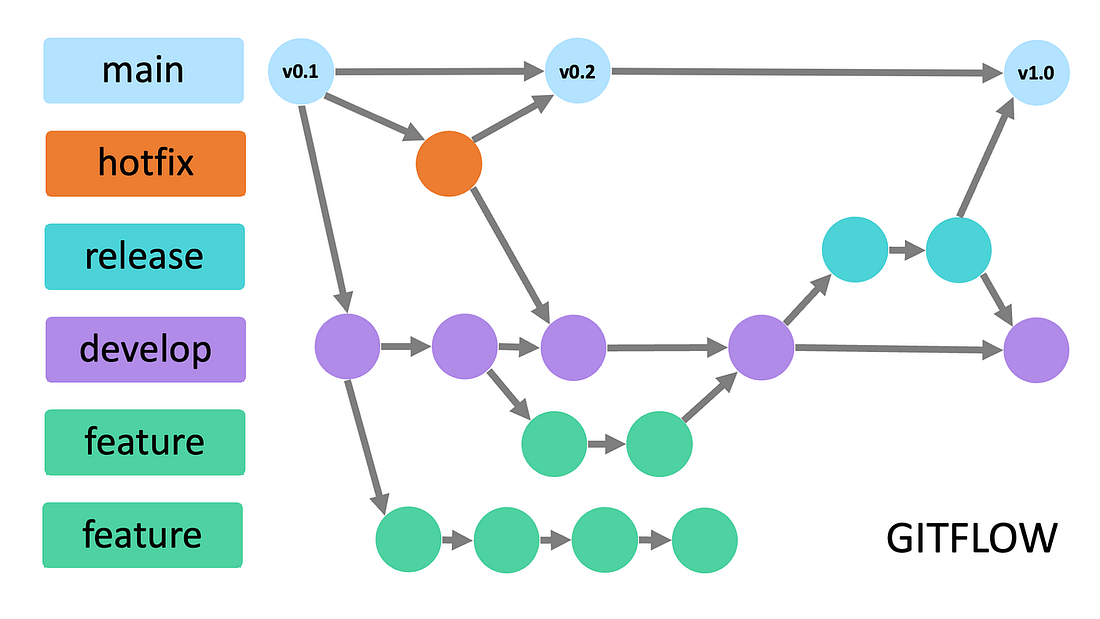
\includegraphics[width=0.8\textwidth]{gitflow_illustration.png}
    \caption[Visualització del GitFlow]{Visualització del GitFlow. Font: \cite{zaghdoudi_secret_nodate}}
    \label{fig:gitflow_illustration}
\end{figure}

Les branques estan dividides de la següent manera:
\begin{itemize}
    \item Feature/\#Numero\_Nom: Branques per realitzar les funcionalitats descrites en la planificació del projecte.
    \item Fix/\#Numero\_Nom: Per solucionar els errors que sorgeixin durant el desenvolupament.
    \item Main: Branca principal, s'utilitza per allotjar les versions testejades i llestes per ser publicades. Cada versió publicada s'etiquetarà seguint el format modul/vX.X (per exemple, backend/v1.0, app/v1.1) per identificar les releases de cada mòdul de forma independent.
    \item Release/\#Numero\_Nom: Branca temporal creada a partir de Dev quan s'acaba un sprint, destinada a estabilitzar i testejar la versió abans de ser fusionada a Main.
    \item Dev: Branca de desenvolupament, integra totes les funcionalitats implementades.
\end{itemize}

\newpage

\section{Planificació temporal}
Per poder limitar i gestionar correctament el temps donat per realitzar el projecte, es realitza una planificació dividida en tasques detallades distribuïdes des del 18/02/2026 fins al 20/06/2026, cobrint un total de 540 hores com és esperat en un treball de fi de grau.

Resulta doncs, en una durada total de quatre mesos i mig amb unes 30 hores setmanals de dedicació necessària. Aquestes 30 hores es repartiran en 4 hores diàries durant dilluns, dimarts, dimecres i dijous, i 7 hores diàries durant dissabte i diumenge. No es poden dedicar més hores entre setmana ja que l'autor del projecte treballa a jornada parcial.
\subsection{Tasques}
\subsubsection{Tasques de gestió del projecte (GP)}
\begin{itemize}
    \item \textbf{GP1 - Contextualització i abast (25 h):} Redacció i maquetació de la primera entrega de GEP, on es descriu el problema que vol solucionar el projecte i quins objectius té. A més, inclou una anàlisi del mercat. Dependències: ---
    \item \textbf{GP2 - Planificació temporal (10 h):} Realització de la planificació del projecte, incloent les tasques a realitzar amb una descripció i la seva especificació per hores, recursos i dependències. Dependències: GP1
    \item \textbf{GP3 - Gestió econòmica i sostenibilitat (15 h):} Elaboració de la tercera entrega de GEP, un document sobre el pressupost econòmic del projecte i informació sobre la sostenibilitat d'aquest. Dependències: GP2
    \item \textbf{GP4 - Document final (15 h):} Document que compren totes les entregues de GEP unificades. Dependències: GP3
\end{itemize}

\subsubsection{Tasques de desenvolupament (D)}

\paragraph{Incepció (I)}
\begin{itemize}
    \item \textbf{I1 - Especificació de requisits (15 h):} Definir les tasques, creant èpiques i històries d'usuari a la plataforma Taiga. Dependències: ---
    \item \textbf{I2 - Definició de l'arquitectura del software (15 h):} Definir a alt nivell (tecnologies, plataformes) el sistema i realitzar un diagrama conceptual. Dependències: I1
    \item \textbf{I3 - Configuració dels entorns (10 h):} Configuració dels entorns de desenvolupament del backend, web i mòbil, assegurant la comunicació entre els tres sistemes. Dependències: I1
\end{itemize}

\paragraph{Sistema d'usuaris i seguretat (SUS)}
\begin{itemize}
    \item \textbf{SUS1 - Autenticació dels usuaris (20 h):} Creació d'un sistema d'autenticació pels usuaris externs, siguin de protectores o possibles adoptants. Dependències: I3
    \item \textbf{SUS2 - Convidar i donar d'alta nous membres (10 h):} Permetre als gestors de protectores convidar a nous membres a unir-se a l'organització. Dependències: SUS1
    \item \textbf{SUS3 - Gestió de rols i permisos (15 h):} Configurar els rols i els permisos del sistema i crear una vista d'admin. Dependències: SUS1
\end{itemize}

\paragraph{Gestió d'animals (GA)}
\begin{itemize}
    \item \textbf{GA5 - Alta i ubicació de l'animal (25 h):} Permetre a un gestor de la protectora registrar un nou animal al sistema, ubicant-lo a un refugi. Dependències: SUS3
    \item \textbf{GA1 - Publicació del perfil d'adopció (10 h):} Permetre a un gestor de la protectora ficar un animal en adopció, configurant-li un perfil públic. Dependències: SUS3, GA5
    \item \textbf{GA4 - Visualització d'animals (15 h):} Vista per visualitzar els animals d'una protectora, amb indicacions de cada un. Dependències: GA5
    \item \textbf{GA2 - Tasques de l'animal (15 h):} Veure quines tasques hi ha pendents per a un cert animal en un interval de dates.. Dependències: GA4
    \item \textbf{GA3 - Gestió del registre mèdic de l'animal (20 h):} Registrar i visualitzar les visites mèdiques i medicacions d'un animal. Dependències: GA5
\end{itemize}

\paragraph{Portal d'adopcions (PA)}
\begin{itemize}
    \item \textbf{PA1 - Llistat d'animals (15 h):} Crea una vista per poder visualtizar els animals filtrant per protectores i altres característiques. Dependències: I3
    \item \textbf{PA2 - Fitxa detallada d'animal (15 h):} Vista per cada animal on es podrà veure els seus detalls i iniciar el procés d'adopció. Dependències: PA1
\end{itemize}

\paragraph{Gestió del procés d'adopció (GPA)}
\begin{itemize}
    \item \textbf{GPA1 - Iniciar adopció (15 h):} Implementació del flux d'adopció, permetent a un adoptant començar una sol·licitud des del portal públic i a un gestor gestionar-ne l'estat. Dependències: PA2, SUS3
    \item \textbf{GPA3 - Generació de contracte d'adopció (20 h):} Crear un mètode de generació automàtica dels contractes d'adopció per als animals. Dependències: GPA1
    \item \textbf{GPA2 - Signatura digital del contracte d'adopció (20 h):} Permetre signar digitalment un contracte d'adopció per part de la protectora. Dependències: GPA3
    \item \textbf{GPA4 - Gestió centralitzada de sol·licituds (15 h):} Implementar una vista a l'aplicació per visualitzar les sol·licituds d'adopció i el seu estat. Dependències: GPA1
\end{itemize}

\paragraph{Gestió de voluntaris i torns (GVT)}
\begin{itemize}
    \item \textbf{GVT1 - Calendari inscripció de torns (25 h):} Implementar un calendari per als voluntaris i gestors de la protectora que permet inscriure's en certes franges. Dependències: SUS3
    \item \textbf{GVT2 - Llistat de tasques del torn (15 h):} Crear una vista per visualitzar les tasques en un cert torn. Dependències: GVT1, GA2
    \item \textbf{GVT3 - Validació d'activitats (15 h):} Permetre als voluntaris veure i completar les tasques acomplides en els seus torns. Dependències: GVT2
\end{itemize}

\paragraph{Ecosistema col·laboratiu (EC)}
\begin{itemize}
    \item \textbf{EC1 - Marketplace de recursos (20 h):} Implementar un apartat de marketplace de protectores on poder publicar material sobrant o necessari i un contacte. Dependències: SUS3
\end{itemize}

\paragraph{Notificacions (NF)}
\begin{itemize}
    \item \textbf{NF1 - Avisos procés d'adopció (15 h):} Habilitació de notificacions per correu electrònic i a través de l'aplicació quan es rebi o actualitzi una sol·licitud d'adopció. Dependències: GPA1
    \item \textbf{NF2 - Alertes de tasques de voluntaris (15 h):} Crear notificacions per cada tasca per als voluntaris. Dependències: NF1, GVT2
\end{itemize}

\paragraph{Desplegament (DP)}
\begin{itemize}
    \item \textbf{DP1 - Desplegar el servidor backend (10 h):} Desplegar el servidor que funciona com a backend a Railway. Dependències: Totes les tasques de desenvolupament
    \item \textbf{DP2 - Desplegar el servidor web (10 h):} Desplegament de la pàgina web pública a Netlify. Dependències: DP1
\end{itemize}

\subsubsection{Documentació final (DF)}
\begin{itemize}
    \item \textbf{DF1 - Memòria final (50 h):} Redacció i maquetació del document de la memòria final del TFG. Dependències: ---
    \item \textbf{DF2 - Defensa del TFG (15 h):} Preparació i pràctica per la defensa del TFG. Dependències: DF1
    \item \textbf{DF3 - Reunions de seguiment (15 h):} Reunions per avaluar l'estat del projecte durant el seu desenvolupament. Dependències: ---
\end{itemize}
\subsection{Recursos}
En aquesta secció es descriuen els recursos que s'utilitzen a les diverses tasques del projecte. Per l'especificació de les tasques no s'inclouen els recursos materials com un espai de treball i un ordinador, ja que hi son present a totes.
\subsubsection{Recursos humans}
\begin{itemize}
    \item \textbf{[AP]} Autor del projecte: Desenvolupador principal de l'aplicació.
    \item \textbf{[DP]} Directora del projecte: Supervisora acadèmica del TFG.
    \item \textbf{[TG]} Tutor de GEP: Tutor de l'assignatura de Gestió de Projectes.
    \item \textbf{[P]} Protectores: Usuaris reals, font de requisits i feedback.
\end{itemize}

\subsubsection{Recursos de software}
\begin{itemize}
    \item \textbf{[AS]} Android Studio: IDE principal per al desenvolupament de l'aplicació Flutter.
    \item \textbf{[W]} WebStorm: IDE per al desenvolupament del portal web en React.
    \item \textbf{[GH]} GitHub: Control de versions i allotjament del codi font.
    \item \textbf{[GP]} GanttProject: Eina per a la planificació i seguiment del projecte.
    \item \textbf{[OL]} Overleaf: Editor \LaTeX{} online per a la redacció de la memòria del TFG.
    \item \textbf{[DI]} Draw.io: Eina de diagrames per a arquitectura, casos d'ús, etc.
    \item \textbf{[T]} Taiga: Gestió àgil de tasques i seguiment del backlog.
    \item \textbf{[BN]} Bruno \cite{bruno_bruno_nodate}: Client d'API per testejar els endpoints del backend.
    \item \textbf{[RW]} Railway \cite{railway_railway_nodate}: Plataforma de desplegament del backend i base de dades.
    \item \textbf{[CD]} Cloudinary \cite{cloudinary_cloudinary_nodate}: Servei d'emmagatzematge i gestió d'imatges al núvol.
    \item \textbf{[NF]} Netlify \cite{netlify_netlify_nodate}: Plataforma de desplegament del portal web públic.
\end{itemize}

\newpage

\subsection{Estimacions temporals i diagrama de Gantt}
Amb les tasques definides, es pot establir una duració per cada una d'elles i veure el temps total estimat del projecte. A més, per cada tasca s'inclouen els recursos necessaris.

\begin{table}[H]
    \centering
    \footnotesize
    \renewcommand{\arraystretch}{0.9}
    \begin{tabular}{|l|l|c|l|l|}
        \hline
        \rowcolor{oceanblue}
        \textcolor{white}{\textbf{ID}} & \textcolor{white}{\textbf{Tasca}} & \textcolor{white}{\textbf{Duració (h)}} & \textcolor{white}{\textbf{Dependències}} & \textcolor{white}{\textbf{Recursos}} \\
        \hline

        \rowcolor{gray!20}
        \textbf{GP} & \textbf{Gestió del projecte} & \textbf{Total: 65} & & \\
        \hline
        GP1 & Contextualització i abast & 25 & --- & AP, DP, TG, OL, T \\
        \hline
        GP2 & Planificació temporal & 10 & GP1 & AP, TG, GP, OL, T \\
        \hline
        GP3 & Gestió econòmica i sostenibilitat & 15 & GP2 & AP, TG, OL \\
        \hline
        GP4 & Document final & 15 & GP3 & AP, TG, OL \\
        \hline

        \rowcolor{gray!20}
        \textbf{D} & \textbf{Desenvolupament} & \textbf{Total: 395} & & \\
        \hline

        \rowcolor{gray!10}
        \textbf{I} & \textbf{Incepció} & \textbf{Total: 40} & & \\
        \hline
        I1 & Especificació de requisits & 15 & --- & AP, DP, P, OL, T \\
        \hline
        I2 & Definició de l'arquitectura del software & 15 & I1 & AP, OL, DI \\
        \hline
        I3 & Configuració dels entorns & 10 & I1 & AP, AS, W, GH \\
        \hline

        \rowcolor{gray!10}
        \textbf{SUS} & \textbf{Sistema d'usuaris i seguretat} & \textbf{Total: 45} & & \\
        \hline
        SUS1 & Autenticació dels usuaris & 20 & I3 & AP, W, AS, GH, BN \\
        \hline
        SUS2 & Convidar i donar d'alta nous membres & 10 & SUS1 & AP, W, GH, BN \\
        \hline
        SUS3 & Gestió de rols i permisos & 15 & SUS1 & AP, W, AS, GH, BN \\
        \hline

        \rowcolor{gray!10}
        \textbf{GA} & \textbf{Gestió d'animals} & \textbf{Total: 85} & & \\
        \hline
        GA5 & Alta i ubicació de l'animal & 25 & SUS3 & AP, W, AS, GH, BN, CD \\
        \hline
        GA1 & Publicació del perfil d'adopció & 10 & SUS3, GA5 & AP, W, GH, BN, CD \\
        \hline
        GA4 & Visualització d'animals & 15 & GA5 & AP, W, AS, GH, BN \\
        \hline
        GA2 & Tasques de l'animal & 15 & GA4 & AP, AS, GH, BN \\
        \hline
        GA3 & Gestió del registre mèdic de l'animal & 20 & GA5 & AP, W, AS, GH, BN \\
        \hline

        \rowcolor{gray!10}
        \textbf{PA} & \textbf{Portal d'adopcions} & \textbf{Total: 30} & & \\
        \hline
        PA1 & Llistat de gats & 15 & I3 & AP, W, GH, BN, CD \\
        \hline
        PA2 & Fitxa detallada de gat & 15 & PA1 & AP, W, GH, BN, CD \\
        \hline

        \rowcolor{gray!10}
        \textbf{GPA} & \textbf{Gestió del procés d'adopció} & \textbf{Total: 70} & & \\
        \hline
        GPA1 & Iniciar adopció & 15 & PA2, SUS3 & AP, W, GH, BN \\
        \hline
        GPA3 & Generació de contracte d'adopció & 20 & GPA1 & AP, W, GH, BN \\
        \hline
        GPA2 & Signatura digital del contracte & 20 & GPA3 & AP, W, GH, BN \\
        \hline
        GPA4 & Gestió centralitzada de sol·licituds & 15 & GPA1 & AP, W, GH, BN \\
        \hline

        \rowcolor{gray!10}
        \textbf{GVT} & \textbf{Gestió de voluntaris i torns} & \textbf{Total: 55} & & \\
        \hline
        GVT1 & Calendari inscripció de torns & 25 & SUS3 & AP, W, AS, GH, BN \\
        \hline
        GVT2 & Llistat de tasques del torn & 15 & GVT1, GA2 & AP, AS, GH, BN \\
        \hline
        GVT3 & Validació d'activitats & 15 & GVT2 & AP, AS, GH, BN \\
        \hline

        \rowcolor{gray!10}
        \textbf{EC} & \textbf{Ecosistema col·laboratiu} & \textbf{Total: 20} & & \\
        \hline
        EC1 & Marketplace de recursos & 20 & SUS3 & AP, W, AS, GH, BN \\
        \hline

        \rowcolor{gray!10}
        \textbf{NF} & \textbf{Notificacions} & \textbf{Total: 30} & & \\
        \hline
        NF1 & Avisos procés d'adopció & 15 & GPA1 & AP, AS, GH, BN \\
        \hline
        NF2 & Alertes de tasques de voluntaris & 15 & NF1, GVT2 & AP, AS, GH, BN \\
        \hline

        \rowcolor{gray!10}
        \textbf{DP} & \textbf{Desplegament} & \textbf{Total: 20} & & \\
        \hline
        DP1 & Desplegar el servidor backend & 10 & Totes les DEV & AP, RW, GH, CD \\
        \hline
        DP2 & Desplegar el servidor web & 10 & DP1 & AP, NF, GH \\
        \hline

        \rowcolor{gray!20}
        \textbf{DF} & \textbf{Documentació final} & \textbf{Total: 80} & & \\
        \hline
        DF1 & Memòria final & 50 & --- & AP, DI, OL \\
        \hline
        DF2 & Defensa del TFG & 15 & DF1 & AP, DI \\
        \hline
        DF3 & Reunions de seguiment & 15 & --- & AP, DI \\
        \hline

        \rowcolor{oceanblue}
        \multicolumn{2}{|l|}{\textcolor{white}{\textbf{Total}}} & \textcolor{white}{\textbf{540 h}} & & \\
        \hline
    \end{tabular}
    \caption[Taula de tasques]{Taula de tasques del projecte. Font: Elaboració pròpia}
    \label{tab:tasques}
\end{table}
Les tasques estan dividides per èpiques, com s'ha mencionat anteriorment, i si es suma la durada total s'obtenen les 540 h previstes per a un treball de fi de grau. 

Observem a continuació el diagrama de Gantt, destacant les dependències entre les tasques, realitzat amb GanttProject \cite{bard_software_sro_ganttproject_nodate}. En aquest cas, la paral·lelització més notable és la de la realització de la memòria amb el desenvolupament del sistema. A causa del temps diari limitat, la resta de tasques són més difícils de paral·lelitzar.
\begin{figure}[H]
    \centering
    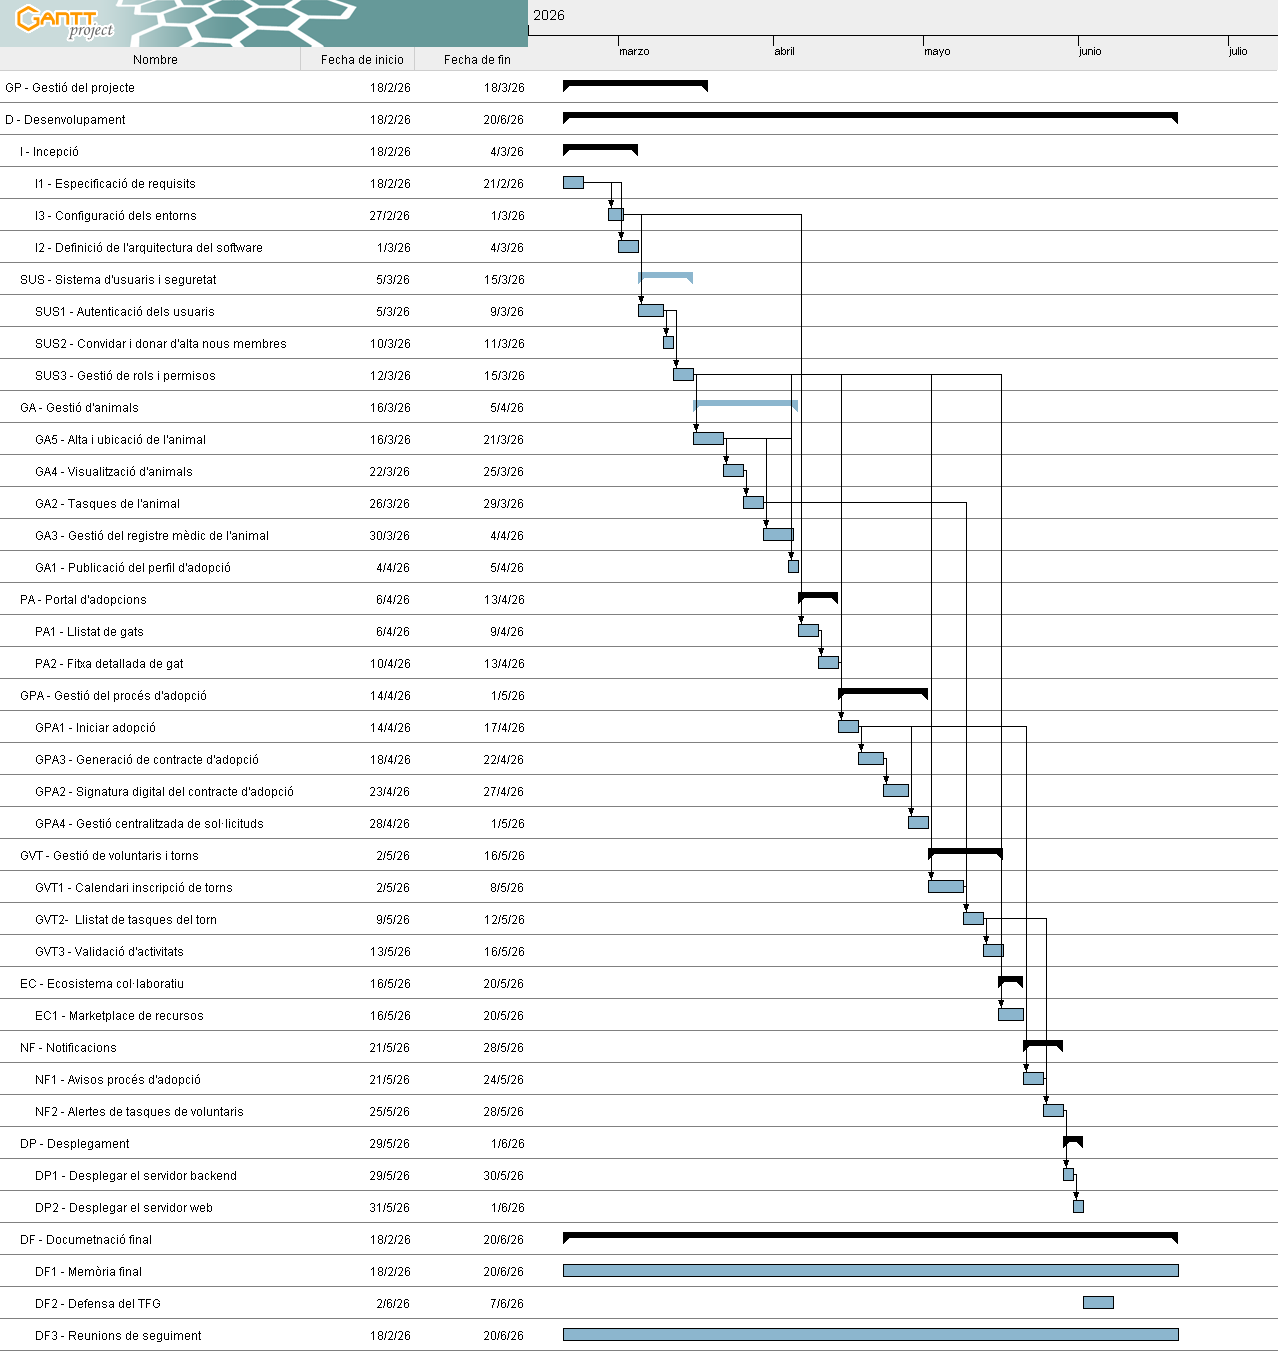
\includegraphics[width=\textwidth]{gant_planif.png}
    \caption[Diagrama de Gantt]{Diagrama de Gantt. Font: Elaboració pròpia}
    \label{fig:gitflow_illustration}
\end{figure}
\newpage
\section{Gestió del risc}
Durant el projecte poden sorgir riscs i obstacles que dificultin el seu desenvolupament, augmentant el nombre d'hores de les tasques o impossibilitant algunes. És per això que en aquesta secció s'especifíquen quins riscos es poden trobar i com es tractaran.

Per cada risc es definirà el seu impacte i la seva probabilitat estimada de què es donin durant el TFG.

\subsection{Data límit d'entrega}
La data d'entrega del TFG és un risc present a qualsevol projecte acadèmic. La probabilitat que afecti al projecte és \textbf{alta} (70--90\%), ja que és habitual que la planificació realitzada inicialment sigui optimista. L'impacte és \textbf{mitjà}, ja que no compromet el sistema sencer sinó funcionalitats secundàries fora del nucli principal. Per mitigar-ho, es treballarà amb un enfocament MVP, prioritzant les funcionalitats nucli i deixant les secundàries com a millores opcionals.

\subsection{Manca d'accés a usuaris reals per validació}
La impossibilitat de treballar directament amb una protectora durant el desenvolupament pot generar un sistema que no s'adapti del tot a les necessitats reals. La probabilitat és \textbf{mitjana} (40--60\%), ja que es disposa d'un estudi previ. L'impacte és \textbf{alt}, perquè podria afectar la utilitat real del producte. Com a mesura de mitigació, s'ha realitzat un anàlisi previ de solucions existents i del funcionament habitual de les protectores.

\subsection{Falta d'experiència amb les tecnologies}
L'autor té experiència limitada amb algunes de les tecnologies utilitzades, especialment en arquitectures multiplataforma. La probabilitat és \textbf{alta} (60--80\%), ja que és el primer projecte d'aquesta escala amb aquest stack. L'impacte és \textbf{alt}, perquè pot generar endarreriments significatius. Per mitigar-ho, es prioritizarà el familiaritzar-se amb les tecnologies el més abans possible i realitzar proves de concepte per entendre les funcionalitats.

\subsection{Bugs i errors de desenvolupament}
L'aparició de bugs durant el desenvolupament és inevitable en qualsevol projecte de software. La probabilitat és \textbf{molt alta} (90--100\%) i l'impacte és \textbf{alt}, ja que poden bloquejar tasques dependents i alterar la planificació. Per mitigar-ho, es faran tests de les funcionalitats principals a mesura que es desenvolupin, evitant acumular problemes cap al final del desenvolupament.

\section{Gestió econòmica}
\label{sec:gestio_economica}
\subsection{Identificació i Estimació de Costos}

Per realitzar aquest estudi suposarem que el projecte el desenvolupen 6 persones cobrint els rols clau del desenvolupament de software, enlloc de l'únic autor del TFG. Aquests rols seran: Project Lead (PL), Arquitecte de Software (AS), Dissenyador UX/UI (DU), Tester (TE) i Enginyer de Software (ES).

\subsubsection{Costos de personal per activitat}

A la Taula \ref{tab:salaris} es mostren els salaris de cada rol segons Glassdoor \cite{glassdoor_salaris_nodate}. S'ha buscat el sou mitjà brut a Espanya, per qualsevol rang d'anys d'experiència:

\begin{table}[H]
    \centering
    \small
    \renewcommand{\arraystretch}{2}
    \begin{tabular}{|l|c|c|}
        \hline
        \rowcolor{oceanblue}\textcolor{white}{\textbf{Rol}} & \textcolor{white}{\textbf{Sou (€/h)}} & \textcolor{white}{\textbf{Sou + SS (€/h)}} \\
        \hline
        Project Lead            & 21,63 & 28,12 \\
        \hline
        Arquitecte de Software  & 24,04 & 31,25 \\
        \hline
        Dissenyador UX/UI       & 13,46 & 17,49 \\
        \hline
        Software Tester         & 11,54 & 15,00 \\
        \hline
        Enginyer de Software    & 12,98 & 16,87 \\
        \hline
    \end{tabular}
    \caption[Salaris per rol]{Salaris mitjans bruts per rol a Espanya. Font: Elaboració pròpia}
    \label{tab:salaris}
\end{table}

Per estimar el cost de personal per activitat, s'atribuirà a cada rol les seves hores d'implicació per cada tasca i s'utilitzarà el cost per hora prèviament definit com es pot observar a la Taula \ref{tab:costos_personal}.

\begin{table}[H]
    \centering
    \footnotesize
    \renewcommand{\arraystretch}{0.9}
    \begin{adjustbox}{max width=\textwidth}
    \begin{tabular}{|l|l|c|c|c|c|c|c|r|}
        \hline
        \rowcolor{oceanblue}
        \textcolor{white}{\textbf{ID}} &
        \textcolor{white}{\textbf{Tasca}} &
        \textcolor{white}{\textbf{PL (h)}} &
        \textcolor{white}{\textbf{AS (h)}} &
        \textcolor{white}{\textbf{DU (h)}} &
        \textcolor{white}{\textbf{TE (h)}} &
        \textcolor{white}{\textbf{ES (h)}} &
        \textcolor{white}{\textbf{Total (h)}} &
        \textcolor{white}{\textbf{Cost (€)}} \\
        \hline

        \rowcolor{gray!20}
        \textbf{GP} & \textbf{Gestió del projecte} & & & & & & \textbf{65} & \\
        \hline
        GP1 & Contextualització i abast            &  8 & 3 & 2 & --- & 12 & 25 & 556,13 \\
        \hline
        GP2 & Planificació temporal                &  5 & 2 & 0 & --- &  3 & 10 & 253,71 \\
        \hline
        GP3 & Gestió econòmica i sostenibilitat    &  8 & 2 & 0 & --- &  5 & 15 & 371,81 \\
        \hline
        GP4 & Document final                       &  5 & 2 & 2 & --- &  6 & 15 & 339,30 \\
        \hline

        \rowcolor{gray!20}
        \textbf{I} & \textbf{Incepció} & & & & & & \textbf{40} & \\
        \hline
        I1  & Especificació de requisits           &  4 & 4 & 3 & --- &  4 & 15 & 357,43 \\
        \hline
        I2  & Definició de l'arquitectura          &  2 & 8 & 1 & --- &  4 & 15 & 391,21 \\
        \hline
        I3  & Configuració dels entorns            &  1 & 4 & 0 & --- &  5 & 10 & 237,47 \\
        \hline

        \rowcolor{gray!20}
        \textbf{SUS} & \textbf{Sistema d'usuaris i seguretat} & & & & & & \textbf{45} & \\
        \hline
        SUS1 & Autenticació dels usuaris           &  1 & 3 & 1 &  3 & 12 & 20 & 386,80 \\
        \hline
        SUS2 & Convidar i donar d'alta membres     &  1 & 1 & 1 &  2 &  5 & 10 & 191,21 \\
        \hline
        SUS3 & Gestió de rols i permisos           &  1 & 2 & 1 &  3 &  8 & 15 & 288,07 \\
        \hline

        \rowcolor{gray!20}
        \textbf{GA} & \textbf{Gestió d'animals} & & & & & & \textbf{85} & \\
        \hline
        GA5  & Alta i ubicació de l'animal         &  1 & 2 & 3 &  3 & 16 & 25 & 458,01 \\
        \hline
        GA1  & Publicació del perfil d'adopció     &  1 & 1 & 3 &  2 &  3 & 10 & 192,45 \\
        \hline
        GA4  & Visualització d'animals             &  1 & 2 & 3 &  2 &  7 & 15 & 291,18 \\
        \hline
        GA2  & Tasques de l'animal                 &  1 & 2 & 2 &  2 &  8 & 15 & 290,56 \\
        \hline
        GA3  & Registre mèdic de l'animal          &  1 & 3 & 2 &  3 & 11 & 20 & 387,42 \\
        \hline

        \rowcolor{gray!20}
        \textbf{PA} & \textbf{Portal d'adopcions} & & & & & & \textbf{30} & \\
        \hline
        PA1  & Llistat de gats                     &  1 & 1 & 3 &  2 &  8 & 15 & 276,80 \\
        \hline
        PA2  & Fitxa detallada de gat              &  1 & 1 & 4 &  2 &  7 & 15 & 277,42 \\
        \hline

        \rowcolor{gray!20}
        \textbf{GPA} & \textbf{Gestió del procés d'adopció} & & & & & & \textbf{70} & \\
        \hline
        GPA1 & Iniciar adopció                     &  1 & 2 & 2 &  2 &  8 & 15 & 290,56 \\
        \hline
        GPA3 & Generació de contracte d'adopció    &  1 & 3 & 2 &  3 & 11 & 20 & 387,42 \\
        \hline
        GPA2 & Signatura digital del contracte     &  1 & 3 & 1 &  3 & 12 & 20 & 386,80 \\
        \hline
        GPA4 & Gestió sol·licituds centralitzada   &  2 & 2 & 2 &  2 &  7 & 15 & 301,81 \\
        \hline

        \rowcolor{gray!20}
        \textbf{GVT} & \textbf{Gestió de voluntaris i torns} & & & & & & \textbf{55} & \\
        \hline
        GVT1 & Calendari inscripció de torns       &  1 & 2 & 4 &  3 & 15 & 25 & 458,63 \\
        \hline
        GVT2 & Llistat de tasques del torn         &  1 & 2 & 2 &  2 &  8 & 15 & 290,56 \\
        \hline
        GVT3 & Validació d'activitats              &  1 & 2 & 1 &  3 &  8 & 15 & 288,07 \\
        \hline

        \rowcolor{gray!20}
        \textbf{EC} & \textbf{Ecosistema col·laboratiu} & & & & & & \textbf{20} & \\
        \hline
        EC1  & Marketplace de recursos             &  2 & 3 & 3 &  3 &  9 & 20 & 399,29 \\
        \hline

        \rowcolor{gray!20}
        \textbf{NF} & \textbf{Notificacions} & & & & & & \textbf{30} & \\
        \hline
        NF1  & Avisos procés d'adopció             &  1 & 2 & 1 &  2 &  9 & 15 & 289,94 \\
        \hline
        NF2  & Alertes tasques voluntaris          &  1 & 2 & 1 &  2 &  9 & 15 & 289,94 \\
        \hline

        \rowcolor{gray!20}
        \textbf{DP} & \textbf{Desplegament} & & & & & & \textbf{20} & \\
        \hline
        DP1  & Desplegar servidor backend          &  1 & 4 & 0 &  2 &  3 & 10 & 233,73 \\
        \hline
        DP2  & Desplegar servidor web              &  1 & 2 & 0 &  2 &  5 & 10 & 204,97 \\
        \hline

        \rowcolor{gray!20}
        \textbf{DF} & \textbf{Documentació final} & & & & & & \textbf{80} & \\
        \hline
        DF1  & Memòria final                       & 15 & 5 & 8 & --- & 22 & 50 & 1.089,11 \\
        \hline
        DF2  & Defensa del TFG                     &  8 & 3 & 2 & --- &  2 & 15 & 387,43 \\
        \hline
        DF3  & Reunions de seguiment               &  8 & 3 & 1 & --- &  3 & 15 & 386,81 \\
        \hline

        \rowcolor{oceanblue}
        \multicolumn{7}{|l|}{\textcolor{white}{\textbf{Total}}} &
        \textcolor{white}{\textbf{540 h}} &
        \textcolor{white}{\textbf{11.232,05 €}} \\
        \hline
    \end{tabular}
    \end{adjustbox}
    \caption[Costos de personal per tasca]{Costos de personal per tasca. Font: Elaboració pròpia}
    \label{tab:costos_personal}
\end{table}

\subsubsection{Costos de Software}
El software utilitzat en aquest projecte no comporta cap cost, degut a que s’utilitza la versió gratuïta. Els serveis de tercers, com les plataformes per desplegar al núvol tampoc, perquè es farà ús del pla gratuït.

\subsubsection{Costos de Hardware}

L'amortització de cada element de Hardware es calcula segons la següent fórmula:

\begin{equation}
    \text{Amortització} = \frac{\text{Preu adquisició}}{\text{Vida útil (anys)}} 
    \times \text{Duració del projecte (anys)}
    \label{eq:amortitzacio}
\end{equation}

Considerant una duració del projecte de 4,5 mesos (0,375 anys), una vida útil de 
6 anys per a l'ordinador i de 5 anys per als perifèrics, s'obtenen els resultats de la Taula \ref{tab:hardware}.

\begin{table}[H]
    \centering
    \small
    \renewcommand{\arraystretch}{2}
    \begin{adjustbox}{max width=\textwidth}
    \begin{tabular}{|l|c|c|c|c|}
        \hline
        \rowcolor{oceanblue}
        \textcolor{white}{\textbf{Element}} &
        \textcolor{white}{\textbf{Preu (€)}} &
        \textcolor{white}{\textbf{Vida útil (anys)}} &
        \textcolor{white}{\textbf{Duració projecte (anys)}} &
        \textcolor{white}{\textbf{Amortització (€)}} \\
        \hline
        Ordinador: Propi                    & 1.450,00 & 6 & 0,375 &  90,62 \\
        \hline
        Ratolí: GXT 922W                    &    25,00 & 5 & 0,375 &   1,88 \\
        \hline
        Teclat: AUKEY KM-G6                 &    40,00 & 5 & 0,375 &   3,00 \\
        \hline
        Pantalla: LG UltraGear 27G610A-B    &   180,00 & 5 & 0,375 &  13,50 \\
        \hline
        \rowcolor{gray!20}
        \textbf{Total} & \textbf{1.695,00} & --- & --- & \textbf{109,00} \\
        \hline
    \end{tabular}
    \end{adjustbox}
    \caption[Costos de Hardware]{Costos de Hardware i amortització. Font: Elaboració pròpia}
    \label{tab:hardware}
\end{table}

\subsubsection{Costos d'espai}

El desenvolupament del projecte s'ha dut a terme des del domicili particular de l'autor, situat a Rubí. Per estimar el cost imputable al projecte, es considera el lloguer mensual del pis, de 1.508 € \cite{enalquilercom_precio_nodate} , durant els 4,5 mesos de duració del projecte. Considerant aquestes dades, el cost total de l'espai es pot veure a la Taula \ref{tab:espai}.

\begin{table}[H]
    \centering
    \small
    \renewcommand{\arraystretch}{2}
    \begin{tabular}{|l|c|c|c|}
        \hline
        \rowcolor{oceanblue}
        \textcolor{white}{\textbf{Concepte}} &
        \textcolor{white}{\textbf{Cost mensual (€)}} &
        \textcolor{white}{\textbf{Duració (mesos)}} &
        \textcolor{white}{\textbf{Cost total (€)}} \\
        \hline
        Lloguer pis (Rubí) & 1.508,00 & 4,5 & 6.786,00 \\
        \hline
        \rowcolor{gray!20}
        \textbf{Total} & \textbf{1.508,00} & \textbf{4,5} & \textbf{6.786,00} \\
        \hline
    \end{tabular}
    \caption[Costos d'espai]{Costos d'espai de treball. Font: Elaboració pròpia}
    \label{tab:espai}
\end{table}


\subsubsection{Costos d'electricitat}
El cost elèctric s'estima a partir del consum en watts de cada dispositiu, 
les hores totals del projecte i el preu mitjà del kWh a Espanya. 
La fórmula utilitzada és:

\begin{equation}
    \text{Cost electricitat} = \frac{\text{Consum (W)}}{1000} 
    \times \text{Hores totals (h)} \times \text{Preu kWh (€)}
    \label{eq:electricitat}
\end{equation}

El consum de l'ordinador s'estima en 500W utilitzant eines online \cite{newegg_power_nodate}, i el de la pantalla LG UltraGear 27G610A-B en 35W, valor típic per a monitors IPS de 27" amb HDR400 en ús normal. 
El preu de referència utilitzat és de 0,1353 €/kWh, corresponent al preu mitjà 
de la tarifa PVPC a Espanya \cite{tarifa_luz_hora_precio_nodate}. Això resulta en els valors de la Taula \ref{tab:electricitat}.

\begin{table}[H]
    \centering
    \small
    \renewcommand{\arraystretch}{2}
    \begin{adjustbox}{max width=\textwidth}
    \begin{tabular}{|l|c|c|c|c|}
        \hline
        \rowcolor{oceanblue}
        \textcolor{white}{\textbf{Dispositiu}} &
        \textcolor{white}{\textbf{Consum (W)}} &
        \textcolor{white}{\textbf{Hores totals (h)}} &
        \textcolor{white}{\textbf{Energia (kWh)}} &
        \textcolor{white}{\textbf{Cost (€)}} \\
        \hline
        Ordinador                       & 500 & 540 & 270,00 & 36,53 \\
        \hline
        Pantalla LG UltraGear 27G610A-B &  35 & 540 &  18,90 &  2,56 \\
        \hline
        \rowcolor{gray!20}
        \textbf{Total} & \textbf{535} & \textbf{540} & \textbf{288,90} & \textbf{39,09} \\
        \hline
    \end{tabular}
    \end{adjustbox}
    \caption[Costos d'electricitat]{Costos d'electricitat del projecte. Font: Elaboració pròpia}
    \label{tab:electricitat}
\end{table}

\subsubsection{Contingències}

Per cobrir possibles desviacions en la planificació, imprevistos tècnics o 
augments no previstos en algun dels costos, s'aplica un marge de contingència 
del 15\% sobre el subtotal de costos directes del projecte. Aquest percentatge ha estat definit a partir de documents de la UPC, on s'informa que el marge es troba entre el 10\% i el 20\%. El resultat es pot veure a la Taula \ref{tab:contingencies}.

\begin{table}[H]
    \centering
    \small
    \renewcommand{\arraystretch}{2}
    \begin{adjustbox}{max width=\textwidth}
    \begin{tabular}{|l|r|r|}
        \hline
        \rowcolor{oceanblue}
        \textcolor{white}{\textbf{Concepte}} &
        \textcolor{white}{\textbf{Cost base (€)}} &
        \textcolor{white}{\textbf{Contingència 15\% (€)}} \\
        \hline
        Costos de personal    & 11.232,05 & 1.684,81 \\
        \hline
        Costos de hardware    &    109,00 &    16,35 \\
        \hline
        Costos d'espai        &  6.786,00 & 1.017,90 \\
        \hline
        Costos d'electricitat &     39,09 &     5,86 \\
        \hline
        \rowcolor{gray!20}
        \textbf{Total contingència} & \textbf{18.166,14} & \textbf{2.724,92} \\
        \hline
    \end{tabular}
    \end{adjustbox}
    \caption[Contingències]{Contingències del projecte (15\%). Font: Elaboració pròpia}
    \label{tab:contingencies}
\end{table}

\subsubsection{Costos dels riscs}

Com s'ha vist a l'apartat de gestió del risc, existeixen diversos riscs que també 
s'han de computar en el cost total. A la Taula~\ref{tab:riscs} veiem per cada risc 
el temps addicional necessari, els rols implicats i la probabilitat d'ocurrència. 
El cost esperat es calcula ponderant el cost brut per la probabilitat mitjana de 
cada risc, obtenint així una estimació més ajustada a la realitat.

\begin{table}[H]
    \centering
    \small
    \renewcommand{\arraystretch}{2}
    \begin{adjustbox}{max width=\textwidth}
    \begin{tabular}{|l|c|c|c|c|c|c|r|c|r|}
        \hline
        \rowcolor{oceanblue}
        \textcolor{white}{\textbf{Risc}} &
        \textcolor{white}{\textbf{PL (h)}} &
        \textcolor{white}{\textbf{AS (h)}} &
        \textcolor{white}{\textbf{DU (h)}} &
        \textcolor{white}{\textbf{TE (h)}} &
        \textcolor{white}{\textbf{ES (h)}} &
        \textcolor{white}{\textbf{Total (h)}} &
        \textcolor{white}{\textbf{Cost brut (€)}} &
        \textcolor{white}{\textbf{Probabilitat}} &
        \textcolor{white}{\textbf{Cost esperat (€)}} \\
        \hline
        Data límit d'entrega               & 5 & 2 & 2 & --- & 11 & 20 & 423,65 & 80\% & 338,92 \\
        \hline
        Manca d'accés a usuaris reals      & 3 & 2 & 5 & --- &  5 & 15 & 318,66 & 50\% & 159,33 \\
        \hline
        Falta d'experiència en tecnologies & 2 & 8 & --- & --- & 15 & 25 & 559,29 & 70\% & 391,50 \\
        \hline
        Bugs i errors de desenvolupament   & 1 & 2 & --- &  8 & 19 & 30 & 531,15 & 95\% & 504,59 \\
        \hline
        \rowcolor{gray!20}
        \textbf{Total} & \textbf{11} & \textbf{14} & \textbf{7} & \textbf{8} & \textbf{50} & \textbf{90} & \textbf{1.832,75} & --- & \textbf{1.394,35} \\
        \hline
    \end{tabular}
    \end{adjustbox}
    \caption[Costos dels riscs]{Costos estimats dels riscs del projecte. Font: Elaboració pròpia}
    \label{tab:riscs}
\end{table}

\subsubsection{Cost total}

La Taula~\ref{tab:cost_total} recull tots els costos identificats al llarg d'aquest 
apartat, incloent els costos directes, les contingències i els costos associats als riscs.

\begin{table}[H]
    \centering
    \small
    \renewcommand{\arraystretch}{2}
    \begin{adjustbox}{max width=\textwidth}
    \begin{tabular}{|l|r|}
        \hline
        \rowcolor{oceanblue}
        \textcolor{white}{\textbf{Concepte}} &
        \textcolor{white}{\textbf{Cost (€)}} \\
        \hline
        Costos de personal (Taula~\ref{tab:costos_personal})     & 11.232,05 \\
        \hline
        Costos de hardware (Taula~\ref{tab:hardware})            &    109,00 \\
        \hline
        Costos d'espai (Taula~\ref{tab:espai})                   &  6.786,00 \\
        \hline
        Costos d'electricitat (Taula~\ref{tab:electricitat})     &     39,09 \\
        \hline
        \rowcolor{gray!20}
        \textbf{Subtotal}                                        & \textbf{18.166,14} \\
        \hline
        Contingències (Taula~\ref{tab:contingencies})            &  2.724,92 \\
        \hline
        Costos dels riscs (Taula~\ref{tab:riscs})                &  1.394,35 \\
        \hline
        \rowcolor{oceanblue}
        \textcolor{white}{\textbf{Total}} &
        \textcolor{white}{\textbf{22.285,41}} \\
        \hline
    \end{tabular}
    \end{adjustbox}
    \caption[Cost total del projecte]{Cost total del projecte. Font: Elaboració pròpia}
    \label{tab:cost_total}
\end{table}

\subsection{Control de gestió}

Al tractar-se d'un projecte de llarga durada, es convenient incorporar una sèrie de mètriques per poder mesurar les desviacions respecte els valors inicials. El resultat d'aquestes mètriques permetrà realitzar canvis a la metodologia i ajustar el que es cregui necessari.

\subsubsection{Mètriques de desviació}

\paragraph{Desviació d'hores}
Mesura si s'està dedicant més o menys temps del previst a una tasca:
\begin{equation}
    \Delta H = H_{\text{estimades}} - H_{\text{reals}}
    \label{eq:desv_hores}
\end{equation}

\paragraph{Desviació del cost per hores treballades}
Quantifica econòmicament la desviació temporal d'una tasca:
\begin{equation}
    \Delta C_H = (H_{\text{estimades}} - H_{\text{reals}}) \times C_{\text{real/hora}}
    \label{eq:desv_cost_hores}
\end{equation}

\paragraph{Desviació en recursos humans per tasca}
Detecta si el cost per hora real ha variat respecte a l'estimat:
\begin{equation}
    \Delta C_{RH} = (C_{\text{estimat/hora}} - C_{\text{real/hora}}) \times H_{\text{reals}}
    \label{eq:desv_rrhh}
\end{equation}

\paragraph{Desviació de costos generals}
Compara els costos indirectes (hardware, espai, electricitat) estimats i reals:
\begin{equation}
    \Delta C_G = C_{G,\text{estimat}} - C_{G,\text{real}}
    \label{eq:desv_generals}
\end{equation}

\paragraph{Desviació de costos imprevistos}
Avalua si les contingències i riscs estimats s'han ajustat a la realitat:
\begin{equation}
    \Delta C_I = C_{I,\text{estimat}} - C_{I,\text{real}}
    \label{eq:desv_imprevistos}
\end{equation}

\paragraph{Desviació total del pressupost}
Mesura global de la diferència entre el pressupost total i el cost final real:
\begin{equation}
    \Delta C_{\text{total}} = C_{\text{pressupost}} - C_{\text{real total}}
    \label{eq:desv_total}
\end{equation}

\subsubsection{Semàfor de control}

Per facilitar la interpretació de les desviacions, s'estableix un sistema de semàfor 
basat en el percentatge de desviació respecte al valor estimat:

\begin{equation}
    \%\Delta = \left| \frac{C_{\text{estimat}} - C_{\text{real}}}{C_{\text{estimat}}} \right| \times 100
    \label{eq:percentatge_desv}
\end{equation}

\begin{table}[H]
    \centering
    \small
    \renewcommand{\arraystretch}{0.8}
    \begin{tabular}{|c|l|l|}
        \hline
        \rowcolor{oceanblue}
        \textcolor{white}{\textbf{Estat}} &
        \textcolor{white}{\textbf{Desviació}} &
        \textcolor{white}{\textbf{Acció}} \\
        \hline
        \cellcolor{green!50}\textbf{VERD}    & $\%\Delta < 10\%$          & Cap acció necessària. \\
        \hline
        \cellcolor{orange!60}\textbf{TARONJA} & $10\% \leq \%\Delta \leq 20\%$ & Revisió de la planificació i avaluar mesures a realitzar. \\
        \hline
        \cellcolor{red!50}\textbf{VERMELL}  & $\%\Delta > 20\%$          & Calen accions immediates i replanificar. \\
        \hline
    \end{tabular}
    \caption[Semàfor de control de desviacions]{Semàfor de control de desviacions. Font: Elaboració pròpia}
    \label{tab:semafar}
\end{table}
\newpage

\section{Especificació}
En aquesta secció es detallarà l'especificació del projecte, incloent els requisits funcionals, dividits per èpiques i històries d'usuari, així com el model conceptual que engloba al sistema.

Els requisits finals descrits a continuació son fruit de l'estudi de mercat realitzat a la secció~\ref{sec:context}, en conjunt amb l'experiència de l'autor realitzant un voluntariat en una protectora d'animals, i la informació recollida a través de contactar amb una entitat de protecció animal local, concretament Rodamons de Rubí \cite{TODO:rodamons}, a través de correu electrònic.

\subsection{Històries d'usuari}
A continuació, es detallen les històries d'usuari agrupades per èpiques, seguint la metodologia Agile. Cada història d'usuari inclou l'objectiu al que fa referència, una descripció clara de la funcionalitat desitjada, els criteris d'acceptació, i una estimació en punts d'esforç basada en la escala de Planning Poker \cite{TODO:planning_poker}, adaptada per a un desenvolupador individual.
\subsubsection{Portal d'adopcions}
Aquesta èpica compren les funcionalitats relacionades amb la pàgina web que actua com a portal d'adopcions per aquells usuaris externs al sistema que volen adoptar un gat. Aquest portal permetrà als usuaris navegar pels gats disponibles per a adopció, veure els seus perfils detallats i iniciar el procés d'adopció.
\HU{RF1}
{Autenticació d'usuaris}
{3}
{5}
{Alta}
{usuari de l'aplicació}
{registrar-me amb el meu número de telèfon mòbil i correu electrònic}
{poder accedir de forma segura a l'aplicació i crear el meu perfil inicial}
{
    \item L'usuari s'ha de registrar amb telèfon i correu.
    \item El sistema envia un codi de verificació per SMS i un altre per email.
    \item L'usuari ha d'introduir ambdós codis per completar el registre.
    \item aasas
}
\subsubsection{Gestió de torns i tasques}

\subsubsection{Procés d'adopció}

\subsubsection{Portal web d'adopcions}

\subsubsection{Comunitat}

\subsubsection{Gestió del compte}

\subsection{Model conceptual}

\subsubsection{Esquema conceptual de classes}

\subsubsection{Descripció de les classes}

\subsubsection{Restriccions d'integritat}

\subsection{Model de comportament}

\subsubsection{Diagrames de seqüència}
\newpage

\section{Disseny}
when displaying a pattern, show maybe diagram + code snippet
\subsection{Descripció general de l'arquitectura}

\subsection{Aplicació mòbil}

\subsubsection{Mockups i disseny visual}

\subsubsection{Navegació}

\subsubsection{Patrons arquitectònics}

\subsubsection{Patrons de disseny}

\subsection{Backend}

\subsubsection{Documentació de l'API}

\subsubsection{Patrons arquitectònics}

\subsubsection{Patrons de disseny}

\subsubsection{Disseny de la base de dades}

\subsection{Portal web d'adopcions}

\subsubsection{Mockups i disseny visual}

\subsubsection{Navegació}

\subsubsection{Patrons arquitectònics}
\newpage

\section{Implementació}
\subsection{Tecnologies utilitzades}
\subsubsection{Backend}
Per crear la part principal del sistema que enllaça tota la resta, el backend, s'ha utilitzat Python com a llenguatge i FastAPI com a framework. Aquesta es una combinació que permet crear 

\subsubsection{Aplicació mòbil}
\subsubsection{Portal web}



\subsection{Anàlisis d'alternatives}
\subsection{Desplegament}
\newpage

\section{Desplegament}
\newpage
\section{Control de qualitat}

\subsection{Tests del backend}

\subsubsection{Tests unitaris}

\subsubsection{Tests d'integració}

\subsection{Tests del frontend}

\subsubsection{Tests de widgets}

\subsubsection{Tests unitaris}

\subsection{Integració i desplegament continus}

\subsubsection{Pipeline de CI}

\subsubsection{Pipeline de CD}
\newpage

\section{Desviacions}
\newpage

\section{Lleis i regulacions}
\newpage

\section{Informe de Sostenibilitat}

\subsection{Autoevaluació}

La sostenibilitat és un concepte que prèviament a aquests exercicis creia que coneixia prou bé per a poder tractar-lo amb profunditat. Després de veure totes les dimensions a les quals pot arribar, he vist que el meu coneixement estava limitat de manera superficial, ja que no considerava el gran impacte de la dimensió econòmica i social de la sostenibilitat.

Com a enginyer del software soc conscient que els projectes que realitzo, tant en l'àmbit professional com en l'acadèmic, tenen un cost ecològic clar. No obstant això, realitzant l'enquesta tinc clar que no conec les eines existents per poder mesurar-ho amb precisió, com ara la petjada ambiental o les matrius d'impacte, ni les he utilitzat mai en cap projecte.

Sobre l'aspecte social, puc afirmar conèixer els conceptes tractats, ja que en alguns cursos laborals es mencionen i estudien. En canvi, pel que fa a la dimensió econòmica, el meu coneixement és més limitat, a causa del fet que tot i haver treballat amb conceptes bàsics de gestió de projectes com pressupostos o diagrames de Gantt, mai he aplicat eines com el DAFO per avaluar la viabilitat econòmica d'un projecte ni he establert una relació amb la sostenibilitat.

Finalment, els aspectes relacionals i ètics sí que els porto a mà en el meu dia a dia. Tinc clara la importància dels diferents interessats en un projecte, i en el cas d'haver de tractar temes ètics, considero que incorporar-los com una variable més és important.

\subsection{Dimensions de la sostenibilitat}

\subsubsection{Dimensió Ambiental}

\textbf{PPP - Has estimat l'impacte ambiental que tindrà la realització del projecte? T'has plantejat minimitzar-lo, per exemple, reutilitzant recursos?}

No s'ha estimat l'impacte ambiental del projecte. Es pot, aproximadament, afirmar que el consum principal del projecte serà el consum elèctric de l'espai de treball. Es planteja minimitzar-lo, ja que tota la feina es centra en un únic ordinador, excepte el desplegament que serà al núvol.

\textbf{Vida útil - Com es resol actualment el problema que vols abordar (estat de l'art)? En què millorarà ambientalment la teva solució respecte a les existents?}

Es resol amb l'ús d'aplicacions similars, i si no és el cas, amb fulls d'Excel o fins i tot amb documents en paper a través de plantilles. En gestionar la protectora a través d'una aplicació, es pot estalviar la necessitat de l'ús de paper tradicional.

\subsubsection{Dimensió Econòmica}

\textbf{PPP - Has estimat el cost de la realització del projecte (recursos humans i materials)?}

Sí, s'ha realitzat una estimació utilitzant el total d'hores planificades pel projecte i costos aproximats. Es pot observar a la Secció \ref{sec:gestio_economica}, on es calcula el cost total a través del Hardware, el Software i els salaris.

\textbf{Vida útil - Com es resol actualment el problema que vols abordar (estat de l'art)? En què millorarà econòmicament la teva solució respecte a les existents?}

Es resol de manera genèrica com la resta de projectes de software. En aquest cas, l'únic avantatge és que es pot prescindir d'alguns càrrecs dins de la gestió del projecte al no ser un equip de moltes persones.

\subsubsection{Dimensió Social}

\textbf{PPP - Què creus que t'aportarà a nivell personal la realització d'aquest projecte?}

Aquest projecte em permetrà millorar les meves habilitats per desenvolupar software escalable, sobretot gestionant un projecte de manera individual i veient el seu cicle de vida de principi a fi. A més, em permetrà entendre les necessitats de les protectores d'animals i desenvolupar la part ètica.

\textbf{Vida útil - Com es resol actualment el problema que vols abordar (estat de l'art)? En què millorarà socialment la teva solució respecte a les existents?}

El meu projecte permetrà portar més fàcilment la gestió d'una protectora, centralitzant la informació i els processos en un únic sistema. En ser una activitat voluntària, un sistema digital que la faciliti i permeti enfocar-se en els principals problemes de les protectores pot resultar molt útil.

\textbf{Vida útil - Existeix una necessitat real del projecte?}

Sí, les protectores són entitats que necessiten d'una gran gestió dels recursos per poder sobreviure. Els animals són cuidats gràcies a persones voluntàries que fan esforços no remunerats per poder ajudar-los. Gràcies al sistema d'aquest projecte es pot conciliar la feina més essencial del dia a dia amb la gestió de totes les variables d'una protectora.

A més, com es menciona a l'apartat del context, existeix un problema respecte l'abandonament d'animals domèstics a Espanya, principalment dels gossos i gats. Aquesta problemàtica es deixa de banda a la societat actual degut a les prioritats dels governs i ciutadans. Un impacte positiu en aquest tema milloraria la qualitat de vida dels animals abandonats i reduiria la càrrega sobre els refugis i protectores.
\newpage
\section{Conclusions}
\newpage
\section{Annexos}

\printbibliography

\end{document}
